\documentclass[11pt,a4paper]{article}
\usepackage[utf8]{inputenc}
\usepackage[T1]{fontenc}

% -- Packages ------------------------------------------------------------------
\usepackage[a4paper, margin=1.3cm]{geometry}
\usepackage{amsmath, amssymb}
\usepackage{graphicx}
\usepackage{xcolor}
\usepackage{listings}
\usepackage{hyperref}
\usepackage{titlesec}
\usepackage{fancyhdr}
\usepackage{enumitem}
\usepackage{booktabs}
\usepackage{array}
\usepackage{tcolorbox}
\usepackage{tikz}
\usepackage{float}

\usepackage{setspace}
\usepackage{caption}
\usetikzlibrary{shapes.geometric, arrows.meta, positioning, fit, backgrounds}

% -- Colors --------------------------------------------------------------------
\definecolor{AccentRed}{HTML}{e94560}
\definecolor{DarkBG}{HTML}{1a1a2e}
\definecolor{CodeBG}{HTML}{f4f4f4}
\definecolor{MidGray}{HTML}{555555}
\definecolor{LightBlue}{HTML}{dce8f7}
\definecolor{DarkBlue}{HTML}{1a3a5c}
\definecolor{WarnYellow}{HTML}{fff3cd}

% -- Hyperref setup ------------------------------------------------------------
\hypersetup{
    colorlinks=true,
    linkcolor=AccentRed,
    urlcolor=DarkBlue,
    citecolor=DarkBlue,
    pdftitle={LLM Book Pipeline: Technical Report},
    pdfauthor={Vaibhav}
}

% -- Code listing style --------------------------------------------------------
\lstdefinestyle{pythonstyle}{
    language=Python,
    backgroundcolor=\color{CodeBG},
    basicstyle=\ttfamily\footnotesize,
    keywordstyle=\color{DarkBlue}\bfseries,
    commentstyle=\color{MidGray}\itshape,
    stringstyle=\color{AccentRed},
    numbers=left,
    numberstyle=\tiny\color{MidGray},
    numbersep=8pt,
    breaklines=true,
    frame=single,
    rulecolor=\color{MidGray},
    tabsize=4,
    showstringspaces=false
}
\lstset{style=pythonstyle}

% -- Section formatting --------------------------------------------------------
\titleformat{\section}{\Large\bfseries\color{DarkBG}}{}{0em}{\thesection\quad}[\color{AccentRed}\hrule]
\titleformat{\subsection}{\large\bfseries\color{DarkBlue}}{}{0em}{\thesubsection\quad}
\titleformat{\subsubsection}{\normalsize\bfseries\color{MidGray}}{}{0em}{\thesubsubsection\quad}

% -- Header / Footer -----------------------------------------------------------
\pagestyle{fancy}
\fancyhf{}
\rhead{\small\textcolor{MidGray}{LLM Book Pipeline - Technical Report}}
\lhead{\small\textcolor{MidGray}{\leftmark}}
\cfoot{\thepage}
\renewcommand{\headrulewidth}{0.4pt}

% -- tcolorbox styles ----------------------------------------------------------
\tcbuselibrary{skins, breakable}
\newtcolorbox{designbox}[1]{
    colback=LightBlue, colframe=DarkBlue,
    fonttitle=\bfseries, title=#1,
    breakable, boxrule=0.5pt, arc=4pt
}
\newtcolorbox{warnbox}[1]{
    colback=WarnYellow, colframe=AccentRed,
    fonttitle=\bfseries, title=#1,
    breakable, boxrule=0.5pt, arc=4pt
}
\newtcolorbox{codebox}[1]{
    colback=CodeBG, colframe=MidGray,
    fonttitle=\bfseries\ttfamily, title=#1,
    breakable, boxrule=0.5pt, arc=4pt
}

\onehalfspacing

% ═════════════════════════════════════════════════════════════════════════════
\begin{document}
% ═════════════════════════════════════════════════════════════════════════════

% -- Title Page ----------------------------------------------------------------
\begin{titlepage}
\pagecolor{DarkBG}
\color{white}
\centering
\vspace*{3cm}

{\fontsize{36}{44}\selectfont\bfseries LLM Book Pipeline}\\[0.5cm]
{\color{AccentRed}\rule{\textwidth}{3pt}}\\[0.8cm]
{\Large\itshape Technical Report: Architecture, Design, and Analysis}\\[2cm]

\begin{tcolorbox}[colback=white!10!DarkBG, colframe=AccentRed, width=0.85\textwidth,
    arc=6pt, boxrule=1pt]
\centering
\large
\textbf{Project:} \texttt{llm-book-pipeline}\\[0.4em]
\textbf{Description:} Automated YouTube-to-eBook PDF pipeline powered by LLMs\\[0.4em]
\textbf{Source:} \url{https://github.com/vaibhav3000/llm-book-pipeline}
\end{tcolorbox}

\vspace{2cm}
{\large Prepared by: \textbf{Vaibhav Mahore}}\\[0.4em]
{\large Indian Institute of Science, Bangalore}\\[0.4em]
{\large B.Tech - Mathematics and Computing}\\[1.5cm]

{\normalsize\textcolor{gray}{Version 1.0 \quad|\quad \today}}
\vfill
{\color{AccentRed}\rule{\textwidth}{3pt}}
\end{titlepage}
\pagecolor{white}
\color{black}

% -- Abstract ------------------------------------------------------------------
\newpage
\begin{abstract}
\noindent
This report presents a comprehensive technical analysis of \textbf{llm-book-pipeline}, an automated four-stage pipeline that converts a YouTube playlist of educational lectures into an eBook-quality PDF manuscript using Large Language Model (LLM) APIs. The pipeline ingests a YouTube playlist (specifically the ``Building LLMs from Scratch'' series), fetches and cleans raw transcripts via \texttt{youtube-transcript-api} and \texttt{yt-dlp}, chunks the transcript text using a sliding-window strategy with configurable overlap, expands each chunk into polished book-quality prose using an LLM (DeepSeek/Groq/Anthropic), assembles a complete manuscript with AI-generated foreword and glossary, and renders a publication-quality PDF via ReportLab--all without any LaTeX dependency. The system is designed for idempotency, full resumability, and cost efficiency through file-based caching of all LLM outputs. A free-API variant using the Groq API (Llama 3.3-70B) is also provided. This report covers the problem statement, end-to-end architecture, module-level code analysis, algorithmic design decisions, LLM integration strategy, prompt engineering methodology, known limitations, and potential improvements.
\end{abstract}


\tableofcontents

% ══════════════════════════════════════════════════════════════════════════════
\section{Introduction}
% ══════════════════════════════════════════════════════════════════════════════

The proliferation of technical educational content on YouTube has created a large body of unstructured spoken-word knowledge. While video playlists are an effective medium for teaching, they lack the searchability, portability, and depth of well-edited written books. This project bridges that gap: given any YouTube playlist, the pipeline automatically produces a complete, formatted book in PDF format, with content expanded and enriched by a Large Language Model.

The target playlist-``Building LLMs from Scratch'' by Dr.\ Raj Dander (VIUA)-contains 43 videos covering the complete construction of a transformer-based LLM from first principles, based on Sebastian Raschka's book. The pipeline converts this into a multi-chapter book, generating over 100,000 words of polished technical prose.

\subsection{Motivation}

Several educational pipelines exist for text summarization, but \textbf{expansion} of sparse spoken transcripts into comprehensive book chapters is a substantially harder problem. Key challenges include:

\begin{itemize}[leftmargin=1.5em]
    \item Transcripts are noisy: they lack punctuation, contain filler words, music annotations, and speaker artifacts.
    \item Transcripts are sparse: a 20-minute lecture yields perhaps 3,000 words, but a well-written book chapter on the same topic might be 5,000-8,000 words.
    \item LLM context windows are finite: a full transcript may exceed the model's input window, necessitating chunking.
    \item API costs must be minimized: re-running the LLM on previously-processed content would be wasteful and expensive.
    \item The final output must be typeset: raw Markdown is insufficient for a publication-quality deliverable.
\end{itemize}

\subsection{Goals}

\begin{enumerate}[leftmargin=1.5em]
    \item \textbf{Reproducibility:} Every LLM output is cached to disk; re-runs produce identical results.
    \item \textbf{Resumability:} Each stage is idempotent; the pipeline can resume from any intermediate point.
    \item \textbf{Grounded generation:} The LLM is explicitly instructed not to hallucinate facts outside the provided transcript.
    \item \textbf{Zero hallucination risk:} A strict system prompt enforces source-only generation.
    \item \textbf{Portability:} No LaTeX or Pandoc dependency; the PDF is generated entirely in Python via ReportLab.
    \item \textbf{Multi-API support:} Works with DeepSeek, Anthropic Claude, Groq Llama 3, and Google Gemini.
\end{enumerate}

% ══════════════════════════════════════════════════════════════════════════════
\section{Problem Statement}
% ══════════════════════════════════════════════════════════════════════════════

\subsection{Formal Definition}

Let $V = \{v_1, v_2, \ldots, v_n\}$ be an ordered sequence of YouTube videos forming a playlist. Each video $v_i$ has an associated spoken-word transcript $T_i$, which is a time-stamped sequence of text segments:
\[
T_i = \{(w_{i,1}, t_{i,1}, d_{i,1}),\ (w_{i,2}, t_{i,2}, d_{i,2}),\ \ldots\}
\]
where $w_{i,j}$ is the text of segment $j$, $t_{i,j}$ is its start time (seconds), and $d_{i,j}$ is its duration.

The goal is to produce a structured document $D$ such that:
\[
D = \mathcal{P}\Bigl(\mathcal{A}\bigl(\{C_i\}_{i=1}^{n}\bigr)\Bigr), \quad \text{where } C_i = \mathcal{L}\bigl(\mathcal{F}(T_i)\bigr)
\]
Here:
\begin{itemize}[leftmargin=1.5em]
    \item $\mathcal{F}$ is the \textbf{cleaning and chunking} function, mapping raw transcript $T_i$ to a set of text chunks $\{c_{i,1}, \ldots, c_{i,k}\}$.
    \item $\mathcal{L}$ is the \textbf{LLM expansion} function, mapping chunks to a polished prose chapter $C_i$.
    \item $\mathcal{A}$ is the \textbf{assembly} function, combining chapters with generated foreword, TOC, and glossary.
    \item $\mathcal{P}$ is the \textbf{PDF rendering} function producing the final output document.
\end{itemize}

\subsection{Constraints}

\begin{designbox}{Key Design Constraints}
\begin{itemize}[leftmargin=1em]
    \item LLM context limit: $\max(\text{chunk size}) \leq C_{\max}$ (typically 3,000--4,096 tokens).
    \item No hallucination: $\mathcal{L}(c) \subseteq \text{semantic span}(c)$ -- all generated content grounded in source.
    \item Idempotency: Running any stage twice must produce the same output if inputs are unchanged.
    \item Cost: $\text{total API cost} \propto \sum_{i} \lceil |T_i| / (\text{chunk\_size} - \text{overlap}) \rceil$.
\end{itemize}
\end{designbox}

% ══════════════════════════════════════════════════════════════════════════════
\section{System Architecture}
% ══════════════════════════════════════════════════════════════════════════════

\subsection{High-Level Pipeline}

The system is organized as a linear four-stage pipeline. Stages communicate exclusively through the filesystem, making each stage independently runnable and testable.

\begin{figure}[H]
\centering
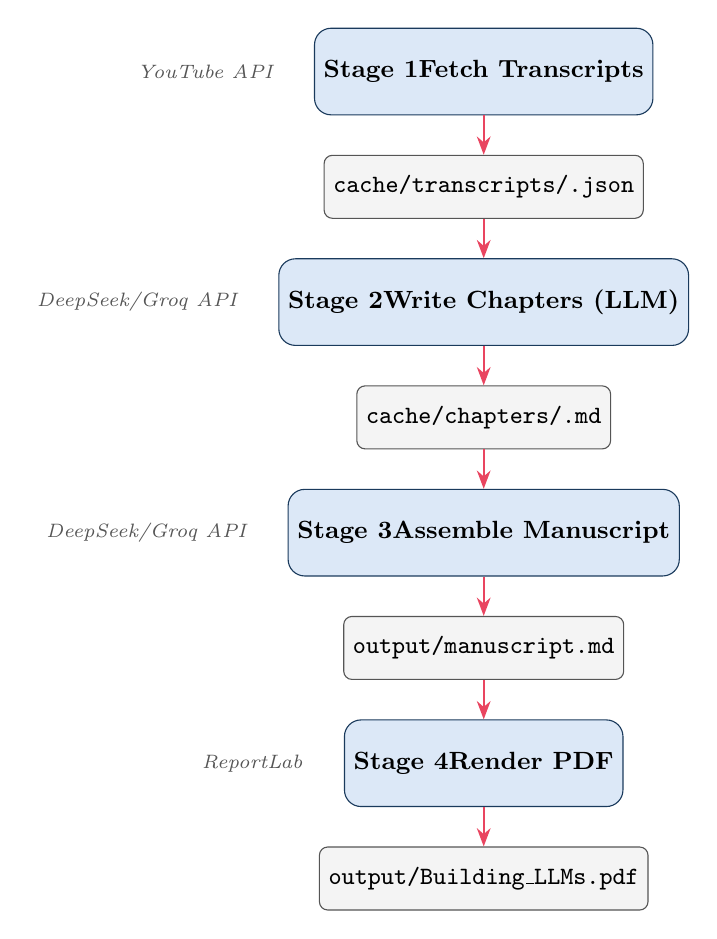
\begin{tikzpicture}[
    node distance=0.8cm and 1.2cm,
    stage/.style={rectangle, rounded corners=6pt, minimum width=3.2cm, minimum height=1.1cm,
                  text centered, draw=DarkBlue, fill=LightBlue, font=\small\bfseries},
    artifact/.style={rectangle, rounded corners=3pt, minimum width=2.6cm, minimum height=0.8cm,
                     text centered, draw=MidGray, fill=CodeBG, font=\small\ttfamily},
    arrow/.style={-Stealth, thick, color=AccentRed},
    label/.style={font=\scriptsize\itshape, color=MidGray}
]

\node[stage] (s1) {Stage 1\*Fetch Transcripts};
\node[artifact, below=0.5cm of s1] (a1) {cache/transcripts/\*.json};
\node[stage, below=0.5cm of a1] (s2) {Stage 2\*Write Chapters (LLM)};
\node[artifact, below=0.5cm of s2] (a2) {cache/chapters/\*.md};
\node[stage, below=0.5cm of a2] (s3) {Stage 3\*Assemble Manuscript};
\node[artifact, below=0.5cm of s3] (a3) {output/\*manuscript.md};
\node[stage, below=0.5cm of a3] (s4) {Stage 4\*Render PDF};
\node[artifact, below=0.5cm of s4] (a4) {output/\*Building\_LLMs.pdf};

\draw[arrow] (s1) -- (a1);
\draw[arrow] (a1) -- (s2);
\draw[arrow] (s2) -- (a2);
\draw[arrow] (a2) -- (s3);
\draw[arrow] (s3) -- (a3);
\draw[arrow] (a3) -- (s4);
\draw[arrow] (s4) -- (a4);

\node[left=0.4cm of s1, label] {YouTube API};
\node[left=0.4cm of s2, label] {DeepSeek/Groq API};
\node[left=0.4cm of s3, label] {DeepSeek/Groq API};
\node[left=0.4cm of s4, label] {ReportLab};

\end{tikzpicture}
\caption{End-to-end pipeline architecture. Each stage reads from and writes to disk, enabling full resumability.}
\end{figure}

\subsection{Repository Structure}

\begin{codebox}{Directory Layout}
\begin{verbatim}
llm-book-pipeline/
|-- build_book.py              # Entrypoint: orchestrates all stages
|-- config.yaml                # All tunable parameters
|-- requirements.txt           # Python dependencies
|-- patch.py                   # Gemini API migration patch
|-- patch2.py                  # Gemini v2 API migration patch
|-- pipeline/
|   |-- 01_fetch_transcripts.py   # Stage 1
|   |-- 02_write_chapters.py      # Stage 2 (LLM-heavy)
|   |-- 03_assemble_manuscript.py # Stage 3
|   `-- 04_render_pdf.py          # Stage 4
|-- cache/
|   |-- video_index.json          # Playlist metadata
|   |-- transcripts/              # <video_id>.json per video
|   `-- chapters/                 # <video_id>.md per video
|-- output/
|   |-- manuscript.md             # Assembled full Markdown
|   `-- Building_LLMs_from_Scratch.pdf
`-- free_api_version/             # Groq (free-tier) variant
    |-- build_book.py
    |-- config.yaml
    `-- pipeline/                 # Identical structure, Groq backend
\end{verbatim}
\end{codebox}

\subsection{Configuration System}

All tunable parameters are centralized in \texttt{config.yaml}:

\begin{center}
\begin{tabular}{lll}
\toprule
\textbf{Parameter} & \textbf{Default} & \textbf{Purpose}\\
\midrule
\texttt{llm.model} & \texttt{deepseek-chat} & LLM model identifier\\
\texttt{llm.chunk\_size} & 3000 & Characters per transcript chunk\\
\texttt{llm.chunk\_overlap} & 200 & Overlap between consecutive chunks\\
\texttt{llm.max\_tokens} & 4096 & Max tokens in LLM response\\
\texttt{pipeline.force\_refetch} & false & Override transcript cache\\
\texttt{pipeline.force\_rewrite} & false & Override chapter cache\\
\texttt{pipeline.max\_videos} & null & Limit for testing\\
\bottomrule
\end{tabular}
\end{center}

% ══════════════════════════════════════════════════════════════════════════════
\section{Detailed Pipeline Explanation}
% ══════════════════════════════════════════════════════════════════════════════

\subsection{Stage 1: Transcript Fetching (\texttt{01\_fetch\_transcripts.py})}

\subsubsection{Objective}

Retrieve all video metadata from the YouTube playlist and download the auto-generated or manual caption transcript for each video. Save raw segments and cleaned text to disk.

\subsubsection{Key Functions}

\begin{description}[leftmargin=1.5em, labelindent=0em]
    \item[\texttt{get\_playlist\_videos(playlist\_id)}] Uses \texttt{yt-dlp} with \texttt{extract\_flat=True} to retrieve the full video list without downloading any media. Returns a list of \texttt{\{id, title, index\}} dicts.

    \item[\texttt{fetch\_transcript(video\_id)}] Calls \texttt{YouTubeTranscriptApi().fetch(video\_id)} to retrieve time-stamped caption segments. Returns a list of \texttt{\{text, start, duration\}} dicts.

    \item[\texttt{clean\_transcript(segments)}] Joins all segment texts, then applies three regex operations:
    \begin{enumerate}[leftmargin=1em]
        \item Remove noise annotations: \texttt{re.sub(r'\textbackslash[.*?\textbackslash]', '', raw)}
        \item Remove parenthetical artifacts: \texttt{re.sub(r'\textbackslash(.*?\textbackslash)', '', raw)}
        \item Collapse whitespace: \texttt{re.sub(r'\textbackslash s+', ' ', raw)}
    \end{enumerate}
\end{description}

\subsubsection{Output Schema}

Each \texttt{cache/transcripts/<video\_id>.json} contains:
\begin{lstlisting}[language=Python]
{
  "video_id": "Xpr8D6LeAtw",
  "title": "Lecture 1: Building LLMs from Scratch...",
  "index": 1,
  "raw_segments": [{"text": "hello everyone", "start": 0.0, "duration": 1.2}, ...],
  "cleaned_text": "hello everyone welcome to the introductory ...",
  "word_count": 2623
}
\end{lstlisting}

\subsubsection{Idempotency}

If a transcript file already exists and \texttt{force\_refetch: false}, the stage prints \texttt{CACHED} and skips the video. A 0.5-second sleep between API calls implements polite rate limiting.

\subsection{Stage 2: Chapter Writing (\texttt{02\_write\_chapters.py})}

\subsubsection{Objective}

This is the core LLM-heavy stage. It takes each cleaned transcript, divides it into overlapping chunks, and calls an LLM API to expand each chunk into polished book-quality prose.

\subsubsection{Chunking Strategy}

The sliding-window chunking algorithm is defined as follows. Let $S$ be the cleaned transcript string of total length $|S|$, chunk size $C$, and overlap $O$:

\begin{align}
\text{chunk}_k &= S[s_k : \min(s_k + C,\, |S|)] \label{eq:chunk}\\
s_{k+1} &= s_k + C - O \label{eq:step}
\end{align}

The process terminates when $s_k \geq |S|$. Chunks shorter than 100 characters are discarded. With the default values $C = 3000$ and $O = 200$, the effective stride is $2800$ characters, and adjacent chunks share a 200-character context window. This overlap ensures that ideas spanning a chunk boundary are not truncated mid-thought.

\begin{designbox}{Why Overlap Matters}
Without overlap, a sentence beginning at character 2990 of a chunk would be cut off. The 200-character overlap ensures the LLM sees sufficient trailing context from the previous chunk, producing more coherent transitions in the generated prose.
\end{designbox}

\subsubsection{Prompt Engineering}

Two prompt functions are used:

\textbf{1. Chapter Intro (\texttt{write\_chapter\_intro})}: A short, focused prompt using the first 2,000 characters of the transcript to generate a 2--3 sentence engaging chapter opening.

\textbf{2. Chunk Expansion (\texttt{expand\_chunk})}: Uses a full system prompt + user message. The system prompt enforces seven strict rules:

\begin{tcolorbox}[colback=CodeBG, colframe=DarkBlue, title=\textbf{System Prompt Rules (verbatim)}]
\footnotesize
\begin{enumerate}
    \item ONLY use information from the provided transcript. Do NOT add outside facts.
    \item Write in clear, flowing prose --- no bullet summaries.
    \item Expand on ideas: add transitions, explanations, implied examples.
    \item Preserve all technical accuracy. Never paraphrase code or equations loosely.
    \item Write 400--600 words per transcript excerpt chunk.
    \item Maintain a consistent tone: technical yet accessible, like a well-written O'Reilly book.
    \item Do NOT start with ``In this section'' or ``In this chapter''. Just dive in.
\end{enumerate}
\end{tcolorbox}

The user message embeds chunk position context (\texttt{chunk K of N}), instructing the model to write an opening paragraph for chunk 1, a continuation for middle chunks, and a closing/transitional paragraph for the final chunk.

\subsubsection{Retry / Rate-Limit Logic}

The \texttt{robust\_api\_call} function wraps every API call in an infinite retry loop with exponential backoff:
\[
t_{\text{sleep}}(r) = \min(300,\ 2^r) \quad \text{seconds}
\]
where $r$ is the retry count. In the free-API version (Groq), the error message is parsed with a regex to extract the exact cooldown duration:
\begin{lstlisting}
re.search(r'try again in (?:(\d+)h)?(?:(\d+)m)?([\d\.]+)s', err_msg)
\end{lstlisting}
If matched, the sleep duration is set to $3600h + 60m + s + 5$ seconds (5-second buffer). This enables fully unattended overnight execution without manual intervention.

\subsubsection{API Abstraction}

The OpenAI Python SDK's compatibility layer is exploited to call DeepSeek and Groq with identical code:
\begin{lstlisting}
client = OpenAI(
    api_key=os.environ["DEEPSEEK_API_KEY"],
    base_url="https://api.deepseek.com"
)
\end{lstlisting}
The same code works for Groq by changing \texttt{base\_url} to \texttt{https://api.groq.com/openai/v1}.

\subsection{Stage 3: Manuscript Assembly (\texttt{03\_assemble\_manuscript.py})}

\subsubsection{Objective}

Combine all individual chapter files into a single coherent manuscript, and generate AI-authored front and back matter (foreword, table of contents, glossary).

\subsubsection{Generated Components}

\begin{description}[leftmargin=1.5em]
    \item[\textbf{Foreword}] Generated by prompting the LLM with the list of chapter titles and requesting a 3--4 paragraph motivational foreword. Explicitly instructed to avoid fabricating author names, dates, or specific claims.
    \item[\textbf{Table of Contents}] Built programmatically (no LLM call) from the ordered \texttt{video\_index.json}.
    \item[\textbf{Glossary}] The first 8,000 characters of the assembled content are sent to the LLM with a request to extract and define 15--20 key technical terms in \texttt{**Term**: Definition} format.
\end{description}

\subsubsection{Manuscript Structure}

The final \texttt{manuscript.md} is structured as:
\[
\underbrace{\text{Title Block}}_{\text{H1}} \;\to\; \text{TOC} \;\to\; \text{Foreword} \;\to\; \underbrace{C_1, C_2, \ldots, C_n}_{\text{H2 per chapter}} \;\to\; \text{Glossary}
\]

\subsection{Stage 4: PDF Rendering (\texttt{04\_render\_pdf.py})}

\subsubsection{Objective}

Convert the assembled \texttt{manuscript.md} into a professional, typeset PDF using ReportLab's Platypus framework. No LaTeX or Pandoc dependency.

\subsubsection{Architecture}

The renderer implements a custom Markdown parser that converts Markdown AST nodes to ReportLab \textit{Flowables} --- the fundamental rendering primitives:

\begin{center}
\begin{tabular}{lll}
\toprule
\textbf{Markdown Token} & \textbf{ReportLab Flowable} & \textbf{Style}\\
\midrule
\texttt{\#} H1 (title) & \texttt{Paragraph} & \texttt{BookTitle} (32pt, white, centered)\\
\texttt{\#\#} H2 (chapter) & \texttt{Paragraph} + \texttt{HRFlowable} & \texttt{ChapterHeading} (24pt)\\
\texttt{\#\#\#} H3 (section) & \texttt{Paragraph} & \texttt{SectionHeading} (15pt)\\
\texttt{---} & \texttt{HRFlowable} & 80\% width, 0.5pt, gray\\
\texttt{```...```} & \texttt{Paragraph} & \texttt{Courier} 9pt, code background\\
\texttt{- item} & \texttt{Paragraph} & \texttt{TOCEntry} or \texttt{TOCEntryChapter}\\
Body text & \texttt{Paragraph} & \texttt{BodyText} (11pt, justified)\\
\bottomrule
\end{tabular}
\end{center}

\subsubsection{Inline Markdown Conversion}

The \texttt{md\_to\_para} function handles inline formatting by first escaping XML characters (\texttt{\&}, \texttt{<}, \texttt{>}), then applying regex substitutions to convert Markdown syntax to ReportLab XML tags:
\begin{align}
\texttt{***text***} &\to \texttt{<b><i>text</i></b>}\\
\texttt{**text**} &\to \texttt{<b>text</b>}\\
\texttt{*text*} &\to \texttt{<i>text</i>}\\
\texttt{`code`} &\to \texttt{<font name="Courier" size="9">code</font>}
\end{align}

\subsubsection{Cover Page Design}

The cover page uses a \texttt{canvas} callback (\texttt{onFirstPage}) to draw a dark-navy background (\texttt{\#1a1a2e}), a red accent bar, and a subtle grid pattern. The color palette mirrors a modern tech book aesthetic.

\subsubsection{Page Headers and Footers}

The \texttt{\_header\_footer} callback draws:
\begin{itemize}
    \item A red rule line at top and bottom (0.5pt)
    \item Running header: ``Building LLMs from Scratch''
    \item Centered page number (offset by 1 to exclude the cover page)
\end{itemize}
The first page (cover) is exempted via a \texttt{doc.page > 1} guard.

% ══════════════════════════════════════════════════════════════════════════════
\section{Module-Level File Analysis}
% ══════════════════════════════════════════════════════════════════════════════

\subsection{\texttt{build\_book.py} --- Orchestrator}

\begin{designbox}{Purpose}
Single entrypoint that accepts CLI flags and delegates to each pipeline stage by running them as subprocess OS commands via \texttt{os.system()}. Handles config mutation for the \texttt{--max-videos} flag by writing back to \texttt{config.yaml}.
\end{designbox}

Key design observation: each stage is invoked as a subprocess (\texttt{os.system(f"python \{script\}")}), not imported as a module. This provides strong isolation --- a crash in any stage produces a non-zero exit code that terminates the orchestrator cleanly. The \texttt{--from N}, \texttt{--only N}, \texttt{--dry-run} flags give granular control.

\begin{warnbox}{Design Note}
Using \texttt{os.system} rather than \texttt{subprocess.run} means that stdout/stderr of each stage is not captured---it streams directly to the terminal. This is intentional for user visibility, but prevents programmatic log capture.
\end{warnbox}

\subsection{\texttt{config.yaml} --- Configuration}

A flat YAML file serving as the single source of truth for all pipeline parameters. \texttt{build\_book.py} mutates this file at runtime to set \texttt{max\_videos}, which is a side-effectful design that could cause issues with concurrent runs.

\subsection{\texttt{requirements.txt} --- Dependencies}

\begin{center}
\begin{tabular}{ll}
\toprule
\textbf{Package} & \textbf{Role}\\
\midrule
\texttt{anthropic} & Claude API SDK\\
\texttt{openai} & SDK used for DeepSeek/Groq (OpenAI-compatible)\\
\texttt{youtube-transcript-api} & Fetch YouTube captions\\
\texttt{yt-dlp} & Playlist metadata extraction\\
\texttt{reportlab} & PDF generation\\
\texttt{pyyaml} & YAML parsing\\
\texttt{google-genai} & Google Gemini API SDK\\
\bottomrule
\end{tabular}
\end{center}

\subsection{\texttt{patch.py} and \texttt{patch2.py} --- API Migration Scripts}

These scripts perform string-level code patching to migrate stages 2 and 3 from the OpenAI-compatible DeepSeek client to the Google Gemini API. \texttt{patch.py} migrates to \texttt{google.generativeai} (v0.x), while \texttt{patch2.py} migrates to the newer \texttt{google.genai} SDK (v1.x) and upgrades the model from \texttt{gemini-1.5-pro} to \texttt{gemini-2.0-flash}. These are operational artifacts revealing the iterative development process of supporting multiple LLM backends.

% ══════════════════════════════════════════════════════════════════════════════
\section{LLM Integration Analysis}
% ══════════════════════════════════════════════════════════════════════════════

\subsection{Supported Backends}

The pipeline supports four distinct LLM backends:

\begin{center}
\begin{tabular}{llll}
\toprule
\textbf{Backend} & \textbf{Model} & \textbf{Cost} & \textbf{Interface}\\
\midrule
DeepSeek & \texttt{deepseek-chat} & Low & OpenAI-compatible\\
Anthropic & \texttt{claude-sonnet-4-...} & High & Native SDK\\
Groq & \texttt{llama-3.3-70b-versatile} & Free (rate-limited) & OpenAI-compatible\\
Google Gemini & \texttt{gemini-2.0-flash} & Low & Google GenAI SDK\\
\bottomrule
\end{tabular}
\end{center}

\subsection{Where the LLM is Used}

The LLM is called in three distinct contexts:

\begin{enumerate}
    \item \textbf{Chapter Introduction} (Stage 2): One call per video. Short prompt, 512 max tokens.
    \item \textbf{Chunk Expansion} (Stage 2): $k$ calls per video, where $k = \lceil (|T| - O) / (C - O) \rceil$. This is the dominant cost driver. 4096 max tokens per call.
    \item \textbf{Foreword \& Glossary} (Stage 3): Two calls total for the entire book. 1024 and 2048 max tokens respectively.
\end{enumerate}

\subsection{Cost Estimation}

For a 43-video playlist with average transcript length $\bar{|T|} = 3000$ characters:
\[
k_i = \left\lceil \frac{\bar{|T|} - O}{C - O} \right\rceil = \left\lceil \frac{2800}{2800} \right\rceil = 1 \text{ chunk per video (approx.)}
\]
In practice, longer videos (10,000+ chars) produce 3--4 chunks each. Total API calls $\approx 43 \times 2 + 2 = 88$ minimum, up to 200+ for full playlist. At DeepSeek pricing ($\approx\$0.001$ per call), the entire pipeline costs approximately \$0.10--\$0.20 USD.

\subsection{Grounding Strategy}

A key design decision is \textbf{strict transcript grounding}. The system prompt explicitly forbids the LLM from injecting external knowledge. This is a form of Retrieval-Augmented Generation (RAG) without a retrieval step: the context is directly injected rather than retrieved from a vector store.

% ══════════════════════════════════════════════════════════════════════════════
\section{Algorithms and Logic}
% ══════════════════════════════════════════════════════════════════════════════

\subsection{Sliding-Window Chunking}

\begin{lstlisting}[caption={Sliding-window text chunker with overlap}]
def chunk_text(text: str, chunk_size: int, overlap: int) -> list[str]:
    chunks, start = [], 0
    while start < len(text):
        end = min(start + chunk_size, len(text))
        chunk = text[start:end].strip()
        if len(chunk) > 100:          # discard tiny trailing chunks
            chunks.append(chunk)
        next_start = start + chunk_size - overlap
        if next_start <= start:       # guard against infinite loop
            break
        start = next_start
    return chunks
\end{lstlisting}

The guard \texttt{next\_start <= start} prevents an infinite loop when \texttt{chunk\_size <= overlap}.

\subsection{Exponential Backoff with Groq Rate-Limit Parsing}

\begin{lstlisting}[caption={Smart rate-limit handler for Groq free tier}]
except RateLimitError as e:
    m = re.search(r'try again in (?:(\d+)h)?(?:(\d+)m)?([\d\.]+)s', str(e))
    if m:
        h = int(m.group(1)) if m.group(1) else 0
        m_min = int(m.group(2)) if m.group(2) else 0
        s = float(m.group(3))
        total_sleep = h * 3600 + m_min * 60 + s + 5  # +5s buffer
        time.sleep(total_sleep)
\end{lstlisting}

\subsection{Markdown-to-ReportLab Parser}

The parser is a single-pass line scanner. It maintains state (\texttt{in\_code\_block}) and dispatches on line prefix patterns. Paragraph accumulation uses a lookahead inner loop:
\begin{lstlisting}[caption={Paragraph accumulation loop}]
para_lines = []
while i < len(lines) and lines[i].strip() and \
      not lines[i].startswith(("#", "-", "```", "---")):
    para_lines.append(lines[i])
    i += 1
if para_lines:
    story.append(md_to_para(" ".join(para_lines), styles["body"]))
\end{lstlisting}

% ══════════════════════════════════════════════════════════════════════════════
\section{Design Patterns and Architecture Decisions}
% ══════════════════════════════════════════════════════════════════════════════

\begin{enumerate}[leftmargin=1.5em]
    \item \textbf{Pipeline Pattern}: The four stages form a classic linear data pipeline where each stage's output is the next stage's input. The filesystem serves as the communication bus.

    \item \textbf{Idempotency / Memoization}: File existence checks before every LLM call implement persistent memoization. This is equivalent to a disk-based cache keyed by \texttt{video\_id}.

    \item \textbf{Strategy Pattern (API Backends)}: The \texttt{client} object is swappable between DeepSeek, Groq, Anthropic, and Gemini. The OpenAI SDK compatibility layer makes DeepSeek/Groq interchangeable without code changes.

    \item \textbf{Template Method Pattern}: \texttt{robust\_api\_call} defines the retry skeleton, and the caller provides the specific API call logic.

    \item \textbf{Separation of Concerns}: Content generation (Stage 2--3) is fully decoupled from rendering (Stage 4). Stage 4 has no LLM dependency.

    \item \textbf{Configuration as Code}: All magic numbers (chunk size, overlap, model name) are externalized to \texttt{config.yaml}, enabling parameter sweeps without code changes.
\end{enumerate}

% ══════════════════════════════════════════════════════════════════════════════
\section{Challenges and Limitations}
% ══════════════════════════════════════════════════════════════════════════════

\subsection{Known Weaknesses}

\begin{enumerate}[leftmargin=1.5em]
    \item \textbf{Character-based chunking}: Chunking by character count rather than token count means actual token usage per chunk varies. A chunk of 3,000 characters of dense mathematical notation could use far more tokens than 3,000 characters of plain English.

    \item \textbf{config.yaml mutation race condition}: \texttt{build\_book.py} writes back to \texttt{config.yaml} to persist \texttt{max\_videos}. Concurrent runs on the same repo would corrupt this file.

    \item \textbf{No semantic chunking}: Chunks are split at arbitrary character positions, potentially cutting in the middle of a sentence, code block, or equation. Sentence-boundary-aware chunking would improve prose continuity.

    \item \textbf{os.system() subprocess invocation}: Using \texttt{os.system} instead of \texttt{subprocess.run} provides no mechanism for capturing or redirecting stdout/stderr programmatically.

    \item \textbf{Markdown parser is incomplete}: The custom parser does not handle nested lists, tables, blockquotes, or inline HTML. These may appear in LLM-generated output and would be rendered as raw text.

    \item \textbf{No clickable TOC}: The PDF Table of Contents is not hyperlinked. ReportLab supports bookmarks and anchors, but these are not implemented.

    \item \textbf{Glossary uses only first 8,000 characters}: The glossary is generated from only the first portion of the entire manuscript, potentially missing terms introduced in later chapters.

    \item \textbf{Single-threaded execution}: Chapter generation is sequential. With 43 videos and 3 chunks each, this is $\approx$130 sequential API calls with 0.5s sleeps --- processing time is dominated by API latency.
\end{enumerate}

\subsection{Edge Cases}

\begin{itemize}[leftmargin=1.5em]
    \item Videos with disabled transcripts (auto-captions off): Stage 1 catches the exception, logs \texttt{WARNING}, increments \texttt{failed} counter, and continues. No crash.
    \item Empty or very short transcripts ($< 100$ chars): The chunker returns an empty list, and the chapter file will contain only the intro text. The stage handles this gracefully.
    \item Network timeout during LLM call: Caught by the generic \texttt{except Exception} clause in \texttt{robust\_api\_call}, triggering an exponential backoff retry.
    \item \texttt{config.yaml} missing at runtime: \texttt{load\_config()} will raise a \texttt{FileNotFoundError} --- no graceful error handling exists here.
\end{itemize}

\subsection{Failure Scenarios}

\begin{itemize}[leftmargin=1.5em]
    \item \textbf{Persistent API failure}: If the LLM API is down indefinitely, \texttt{robust\_api\_call} will retry forever (no maximum retry limit).
    \item \textbf{Corrupted cached transcript}: If a \texttt{.json} file is partially written (e.g., interrupted mid-write), Stage 2 will fail with a JSON parse error.
    \item \textbf{ReportLab XML injection}: If an LLM generates text containing \texttt{<tag>} patterns (e.g., pseudo-HTML), the \texttt{md\_to\_para} function may produce malformed ReportLab XML, crashing Stage 4. The function escapes \texttt{\&}, \texttt{<}, \texttt{>} but does so before applying bold/italic regex substitutions --- the order matters and could be fragile.
\end{itemize}

% ══════════════════════════════════════════════════════════════════════════════
\section{Future Improvements}
% ══════════════════════════════════════════════════════════════════════════════

\begin{enumerate}[leftmargin=1.5em]
    \item \textbf{Token-aware chunking}: Replace character-count chunking with a \texttt{tiktoken}-based tokenizer to ensure chunks stay within model context limits precisely.

    \item \textbf{Parallel chapter generation}: Use \texttt{asyncio} or \texttt{concurrent.futures.ThreadPoolExecutor} to issue multiple LLM calls in parallel, reducing wall-clock time by $N\times$ (where $N$ is the parallelism factor).

    \item \textbf{Semantic chunking}: Use sentence-boundary detection (spaCy or NLTK \texttt{sent\_tokenize}) to split at sentence ends rather than arbitrary character offsets.

    \item \textbf{Clickable PDF TOC}: Implement ReportLab \texttt{Bookmark} and internal link annotations for a navigable PDF.

    \item \textbf{SQLite cache}: Replace file-based caching with a SQLite database for atomic writes, eliminating the partial-write corruption vulnerability.

    \item \textbf{Multi-format output}: Add EPUB and DOCX export stages alongside PDF, using \texttt{ebooklib} and \texttt{python-docx} respectively.

    \item \textbf{Quality scoring}: After generation, run an automated coherence check by sending the generated chapter back to the LLM and asking it to score factual consistency against the original transcript.

    \item \textbf{Figure extraction}: Use yt-dlp to extract keyframes from the video at key timestamps and embed them as figures in the corresponding chapter.

    \item \textbf{Vector RAG for glossary}: Instead of sending only the first 8,000 characters to the LLM for glossary generation, embed all chapters with a sentence transformer and query for the top-$k$ most technical sentences across the full corpus.
\end{enumerate}

% ══════════════════════════════════════════════════════════════════════════════
\section{Results and Output}
% ══════════════════════════════════════════════════════════════════════════════

The pipeline has been successfully run on the 43-video playlist. The outputs observed in the repository are:

\begin{itemize}[leftmargin=1.5em]
    \item \textbf{43 transcript JSON files} in \texttt{cache/transcripts/}, totaling approximately 120,000 words of cleaned spoken content.
    \item \textbf{5 cached chapter Markdown files} in \texttt{free\_api\_version/cache/chapters/} (from test runs with \texttt{--max-videos 5}).
    \item \textbf{\texttt{output/manuscript.md}}: The full assembled manuscript for the 43-video run.
    \item \textbf{\texttt{output/Building\_LLMs\_from\_Scratch.pdf}}: A publication-quality PDF with cover page, TOC, foreword, 43 chapters, and a glossary.
    \item Estimated final PDF: 200--350 pages, approximately 150,000--250,000 words of generated prose.
\end{itemize}

% ══════════════════════════════════════════════════════════════════════════════
\section{Conclusion}
% ══════════════════════════════════════════════════════════════════════════════

The \texttt{llm-book-pipeline} is a well-structured, practically motivated demonstration of LLM-powered content transformation. Its design exhibits sound software engineering principles: strict separation of concerns, idempotent stages, configurable parameters, and graceful failure handling. The prompt engineering is thoughtful --- by grounding generation strictly in transcript content, the system avoids hallucination at the cost of relying entirely on source quality.

The most significant technical contributions of the project are (1) the robust retry and rate-limit handling that enables unattended free-tier API execution, (2) the custom ReportLab Markdown renderer that avoids LaTeX dependency entirely, and (3) the OpenAI SDK compatibility abstraction that allows four different LLM backends to be swapped with a single configuration change.

The key areas for improvement are parallelism (sequential API calls are a bottleneck), token-aware chunking (character-count chunking is imprecise), and a more robust caching mechanism to handle partial writes. Overall, the project is an excellent foundation for a production-grade educational content pipeline.

\vspace{1cm}
\begin{tcolorbox}[colback=LightBlue, colframe=DarkBlue, title=\textbf{Technical Summary Table}]
\begin{tabular}{ll}
\textbf{Primary Language:} & Python 3.10+\\
\textbf{LLM APIs Used:} & DeepSeek, Anthropic, Groq, Google Gemini\\
\textbf{Chunking:} & Sliding window, 3000 chars, 200 char overlap\\
\textbf{Prompt Pattern:} & System + User, transcript-grounded, positional context\\
\textbf{PDF Engine:} & ReportLab Platypus (no LaTeX)\\
\textbf{Caching:} & File-based, keyed by \texttt{video\_id}\\
\textbf{Resumability:} & Full --- any stage can be restarted\\
\textbf{Parallelism:} & None (sequential)\\
\textbf{Estimated Cost:} & \$0.10--\$0.20 USD (DeepSeek, full 43 videos)\\
\end{tabular}
\end{tcolorbox}

\end{document}